\documentclass[12pt]{article}

\usepackage[utf8]{inputenc}
\usepackage[margin=1in]{geometry}
\usepackage{amsmath}
\usepackage{graphicx}
\usepackage{xcolor}
\usepackage{cancel}

\usepackage{listings}
\usepackage{xcolor}

% Python code styling
\lstset{
    language=Python,
    basicstyle=\ttfamily\small,
    numbers=left,
    numberstyle=\tiny,
    stepnumber=1,
    numbersep=5pt,
    backgroundcolor=\color{gray!10},
    showspaces=false,
    showstringspaces=false,
    showtabs=false,
    frame=leftline,
    tabsize=4,
    captionpos=b,
    breaklines=true,
    breakatwhitespace=false,
    title=\lstname,
    keywordstyle=\color{blue},
    stringstyle=\color{orange},
    commentstyle=\color{green!60!black},
    emphstyle=\color{magenta},
    identifierstyle=\color{black}
}

\title{Autumn Term Coursework}
\author{Harsh Agrawal, CID:~02320622}
\date{\today}

\begin{document}

\maketitle

\subsection*{Question 1: Linear model of a cross-catalytic self-replicator}
A system is constructed in which two chemical species, X and Y, each catalyse
the formation of the other from the relevant building blocks. The effective
reactions, treating the building blocks implicitly, are:
\begin{align}
    \text{X} \xrightarrow{r} \text{X} + \text{Y} \nonumber \\
    \text{Y} \xrightarrow{s} \text{Y} + \text{X} \label{eq:1}
\end{align}
Here, $r$ and $s$ are the rate constants of the relevant reactions.

\subsubsection*{a. Write down the ODEs giving $\frac{d[X]}{dt}$ and $\frac{d[Y]}{dt}$ for the system in 1 under the assumption of mass-action kinetics.}

From equations (1a) and (1b), we can see that both X and Y respectively
catalyse the formation of the other entity. Thus, under the assumption of
mass-action kinetics, the ODEs for the system can be written as:
\begin{align*}
    \frac{d[X]}{dt} = s[Y] \\
    \frac{d[Y]}{dt} = r[X]
\end{align*}

\sloppy
\subsubsection*{b. Using the substitutions $\alpha x = X$, $\beta y = Y$ and $\gamma \tau = t$, perform a non-dimensionalization (or renormalization)
    to yield
    \begin{align}
        \frac{dx}{d\tau} & = y \nonumber \\
        \frac{dy}{d\tau} & = x
    \end{align}
    where $\dot{x} = \frac{dx}{d\tau}$ and $\dot{y} = \frac{dy}{d\tau}$.}

Since $t = \gamma \tau$,
\begin{equation*}
    \frac{d\tau}{dt} = \frac{1}{\gamma} \implies \frac{d}{dt} = \frac{d}{d\tau} \frac{d\tau}{dt} = \frac{1}{\gamma} \frac{d}{d\tau} \quad\textcolor{gray}{\text{ (Using chain rule)}}
\end{equation*}

By plugging $\frac{d}{dt} = \frac{1}{\gamma} \frac{d}{d\tau}$, $[X] = \alpha x$
and $[Y] = \beta y$ into the ODEs, we get:
\begin{equation*}
    \begin{aligned}
        \frac{d [X]}{dt} = s[Y] \implies \frac{1}{\gamma} \frac{d (\alpha x)}{d\tau} & = s \beta y                      \\
        \frac{dx}{d\tau}                                                             & = \frac{s\beta \gamma}{\alpha} y
    \end{aligned}
\end{equation*}

\begin{equation*}
    \begin{aligned}
        \frac{d [Y]}{dt} = r[X] \implies \frac{1}{\gamma} \frac{d (\beta y)}{d\tau} & = r \alpha x                     \\
        \frac{dy}{d\tau}                                                            & = \frac{r\alpha \gamma}{\beta} x
    \end{aligned}
\end{equation*}

\noindent
We can perfom non-dimensionalization by arbitrarily setting $\gamma = 1$,
$\alpha = \frac{\beta}{r}$ and $\beta = \frac{\alpha}{s}$ and simplifying the equations above:
\begin{align*}
    \frac{dx}{d\tau} & = \frac{\cancel{s}\cdot(\cancel{\alpha}/\cancel{s})\cdot1}{\cancel{\alpha}}y = y \\
    \frac{dy}{d\tau} & = \frac{\cancel{r}\cdot(\cancel{\beta}/\cancel{r})\cdot1}{\cancel{\beta}}x = x
\end{align*}

\subsubsection*{c. Identify the fixed point $(x^*,y^*)$ for the system in Eq. 2.}

To find fixed points, we set $\frac{dx}{d\tau} = 0$ and $\frac{dy}{d\tau} = 0$.
\begin{align*}
    \frac{dx}{d\tau} = 0 \implies y = 0 \\
    \frac{dy}{d\tau} = 0 \implies x = 0
\end{align*}

\noindent
Thus, the only fixed points in this system are $(x^*,y^*) = (0,0)$.

\subsubsection*{d. Sketch the phase plane of the system in Eq. 2.}
The eigenvectors of the Jacobian were first plotted in the phase plane along which four different trajectories were plotted qualitatively.

\begin{figure}[htbp]
    \centering
    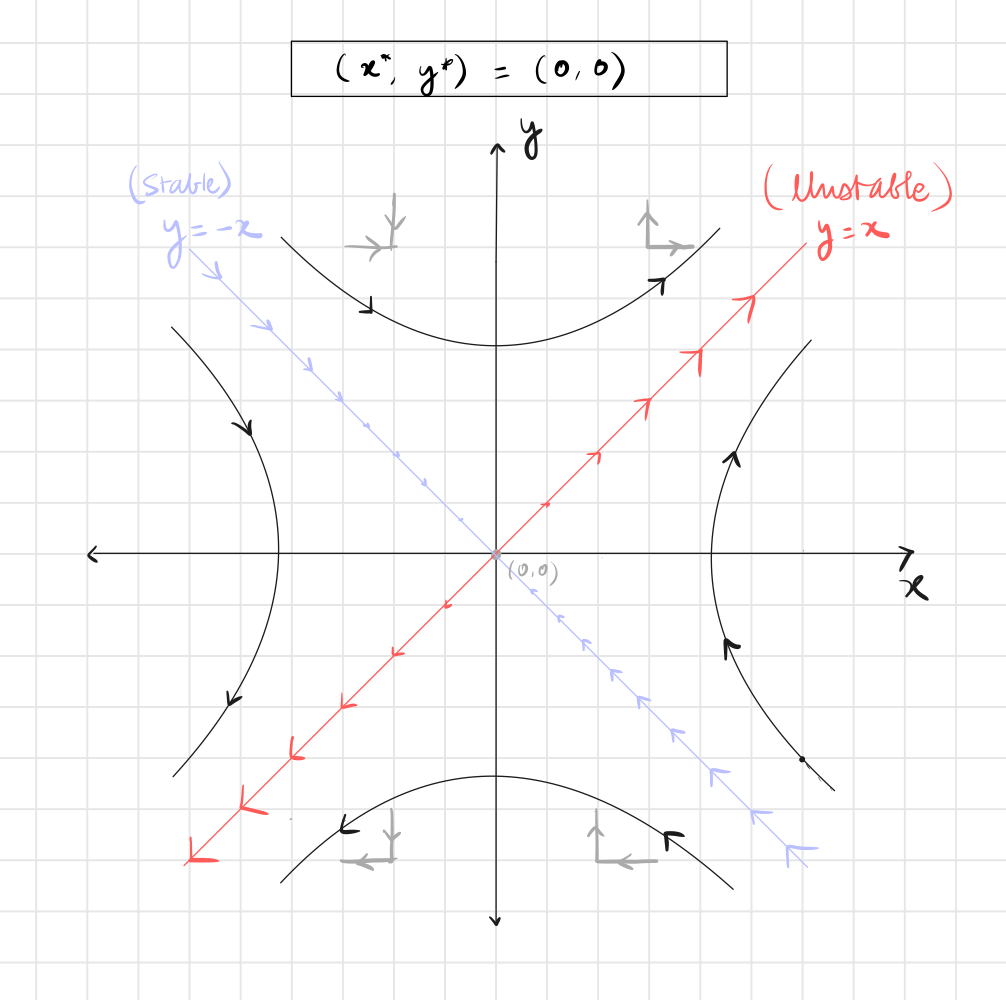
\includegraphics[width=0.6\textwidth]{figures/q1_sketch.jpeg}
    \caption{\centering Phase plane of the system in Eq. 2. The eigenvectors of the Jacobian are plotted in the vicinity of the fixed point $(x^*,y^*) = (0,0)$ and four different trajectories were plotted qualitatively.}
\end{figure}

\newpage
\subsubsection*{e. We now interpret the results in terms of the physical variables [X] and [Y]. Assuming that at least one of [X],[Y] $> 0$ at $t=0$, explain what happens to [X], [Y] and [X]/[Y] as $t \to \infty$.}

From the phase plane, its clear that if either $[X]$ or $[Y]$ is positive at
$t=0$, the system will move away from the fixed point $(x^*,y^*) = (0,0)$ and
towards infinity (exponentially).

\noindent
Mathematically, we can write this as:
\begin{equation*}
    \text{If at } t = 0, [X] > 0 \text{ or } [Y] > 0, \text{ then } \lim_{t \to \infty} [X] = \lim_{t \to \infty} [Y] = \infty
\end{equation*}

For the fraction $\frac{[X]}{[Y]}$,

we can write:
\begin{align*}
    \frac{\frac{d[X]}{dt}}{\frac{d[Y]}{dt}} & = \frac{s[Y]}{r[X]} = \frac{\alpha x}{\beta y}                        \\
    \lim_{t \to \infty} \frac{[X]}{[Y]}     & = \lim_{t \to \infty} \frac{\alpha x}{\beta y} = \frac{\alpha}{\beta}
\end{align*}

Thus, as $t \to \infty$, $\frac{[X]}{[Y]} \to \frac{\alpha}{\beta}$.

\section*{Question 2: A non-linear model of a chemical replicator}
In an attempt to provide a more realistic description of the dynamics for large time, an alternative non-linear
model of the replicator is constructed. The resultant ODE model is
\begin{equation}
    \begin{aligned}
        \dot{x} & = y - x^2  \\
        \dot{y} & = 8x - y^2
    \end{aligned}
    \tag{3}
\end{equation}
In Eq. 3, the value of 8 has been assumed for the only parameter that remains after non-dimensionalization.

\subsubsection*{a. Show that the two physically-relevant fixed points for the system in Eq. 3 are:
    $(x^*,y^*) = (0,0)$,
    $(x^*,y^*) = (2,4)$.}

To find fixed points, we set $\dot{x} = 0$ and $\dot{y} = 0$.
\begin{align*}
    \dot{x} = 0 \implies y = x^2 \\
    \dot{y} = 0 \implies 8x = y^2
\end{align*}

Substituting $y = x^2$ into $8x = y^2$, we get:
\begin{align*}
    8x = {(x^2)}^2 \implies 8x = x^4 \implies x^4 - 8x = 0 \implies x(x^3 - 8) = 0 \\
    \implies x = 0 \text{ or } x = 2
\end{align*}

When $x = 0$:
\begin{align*}
    y = x^2 = 0 \implies (x^*,y^*) = (0,0)
\end{align*}

When $x = 2$:
\begin{align*}
    y = x^2 = 4 \implies (x^*,y^*) = (2,4)
\end{align*}

\subsubsection*{b. By finding eigenvalues of the Jacobian at the fixed points, identify the stability of the fixed points.}

The Jacobian is given by:
\begin{align*}
    J = \begin{pmatrix}
            \frac{\partial \dot{x}}{\partial x} & \frac{\partial \dot{x}}{\partial y} \\
            \frac{\partial \dot{y}}{\partial x} & \frac{\partial \dot{y}}{\partial y}
        \end{pmatrix} = \begin{pmatrix}
                            -2x & 1   \\
                            8   & -2y
                        \end{pmatrix}
\end{align*}

We can evaluate the eigenvalues of $J$ at $(x^*,y^*) = (0,0)$ by solving the
characteristic equation:
\begin{align*}
    \det(J_{(0,0)} - \lambda I) = 0 \implies \begin{vmatrix}
                                                 \begin{pmatrix}
            0 & 1 \\
            8 & 0
        \end{pmatrix} - \lambda \begin{pmatrix}
                                    1 & 0 \\
                                    0 & 1
                                \end{pmatrix}
                                             \end{vmatrix} = 0 \\
    \begin{vmatrix}
        -\lambda & 1        \\
        8        & -\lambda
    \end{vmatrix} = 0 \implies \lambda^2 - 8 = 0 \implies \lambda = \pm \sqrt{8}
\end{align*}

Similarly, for $(x^*,y^*) = (2,4)$:
\begin{align*}
    \det(J_{(2,4)} - \lambda I) = 0 \implies \begin{vmatrix}
                                                 \begin{pmatrix}
            -4 & 1  \\
            8  & -8
        \end{pmatrix} - \lambda \begin{pmatrix}
                                    1 & 0 \\
                                    0 & 1
                                \end{pmatrix}
                                             \end{vmatrix} = 0 \\
    \begin{vmatrix}
        -4-\lambda & 1          \\
        8          & -8-\lambda
    \end{vmatrix} = 0 \implies \lambda^2 + 12\lambda + 24 = 0                                               \\
    \implies \lambda = \frac{-12 \pm \sqrt{144-96}}{2} = -6 \pm \sqrt{12}
\end{align*}
Since both eigenvalues are negative, $(2,4)$ is a stable fixed point. Moreover, since one eigenvalue is positive, the origin $(0,0)$ is an unstable fixed point (saddle point).

\subsubsection*{c. Show that the eigenvectors of the linear system around the fixed points are:
    \[\begin{pmatrix} \delta x \\ \delta y \end{pmatrix} = \begin{pmatrix} 1 \\ 2\sqrt{2} \end{pmatrix} \text{ and } \begin{pmatrix} 1 \\ -2\sqrt{2} \end{pmatrix} \text{ for } (x^*,y^*) = (0,0),\]
    \[\begin{pmatrix} \delta x \\ \delta y \end{pmatrix} = \begin{pmatrix} 1 \\ -2 + 2\sqrt{3} \end{pmatrix} \text{ and } \begin{pmatrix} 1 \\ -2-2\sqrt{3} \end{pmatrix} \text{ for } (x^*,y^*) = (2,4).\]
}

For $(x^*,y^*) = (0,0)$, we found $\lambda = \pm\sqrt{8} = \pm 2\sqrt{2}$.
Let's verify the eigenvectors:

For $\lambda = 2\sqrt{2}$:
\begin{align*}
    (J_{(0,0)} - \lambda I)\vec{v} = \vec{0} \implies \begin{pmatrix}
                                                          -2\sqrt{2} & 1          \\
                                                          8          & -2\sqrt{2}
                                                      \end{pmatrix}\begin{pmatrix}
                                                                       v_1 \\ v_2
                                                                   \end{pmatrix} = \begin{pmatrix}
                                                                                       0 \\ 0
                                                                                   \end{pmatrix}
\end{align*}

This gives us:
\begin{align*}
    -2\sqrt{2}v_1 + v_2 & = 0 \\
    8v_1 - 2\sqrt{2}v_2 & = 0
\end{align*}

Setting $v_1 = 1$, we get $v_2 = 2\sqrt{2}$, confirming the first eigenvector $\begin{pmatrix} 1 \\ 2\sqrt{2} \end{pmatrix}$.

For $\lambda = -2\sqrt{2}$, similar calculations yield the second eigenvector $\begin{pmatrix} 1 \\ -2\sqrt{2} \end{pmatrix}$.

For $(x^*,y^*) = (2,4)$, we found $\lambda = -6 \pm \sqrt{12} = -6 \pm
    2\sqrt{3}$. Let's verify:

For $\lambda = -6 + 2\sqrt{3}$:
\begin{align*}
    (J_{(2,4)} - \lambda I)\vec{v} = \vec{0} \implies \begin{pmatrix}
                                                          -4-(-6+2\sqrt{3}) & 1                 \\
                                                          8                 & -8-(-6+2\sqrt{3})
                                                      \end{pmatrix}\begin{pmatrix}
                                                                       v_1 \\ v_2
                                                                   \end{pmatrix} = \begin{pmatrix}
                                                                                       0 \\ 0
                                                                                   \end{pmatrix}
\end{align*}

This gives us:
\begin{align*}
    (2-2\sqrt{3})v_1 + v_2   & = 0 \\
    8v_1 + (-2-2\sqrt{3})v_2 & = 0
\end{align*}

Setting $v_1 = 1$, we get $v_2 = -2 + 2\sqrt{3}$, confirming the first
eigenvector $\begin{pmatrix} 1 \\ -2+2\sqrt{3} \end{pmatrix}$.

Similarly, for $\lambda = -6 - 2\sqrt{3}$, we obtain the second eigenvector $\begin{pmatrix} 1 \\ -2-2\sqrt{3} \end{pmatrix}$.

\subsubsection*{d. Thus sketch the phase plane of the system in Eq. 3, showing the two fixed points and trajectories in the
    vicinity of those fixed points (the phase plane far away from these points may be left blank).}

Similar to question 1, the eigenvectors of the Jacobian were plotted in the
vicinity of the two fixed points (one stable and one unstable saddle point).
Along these four eigenvectors (two for each fixed point), various different
trajectories were plotted qualitatively.
\begin{figure}[htbp]
    \centering
    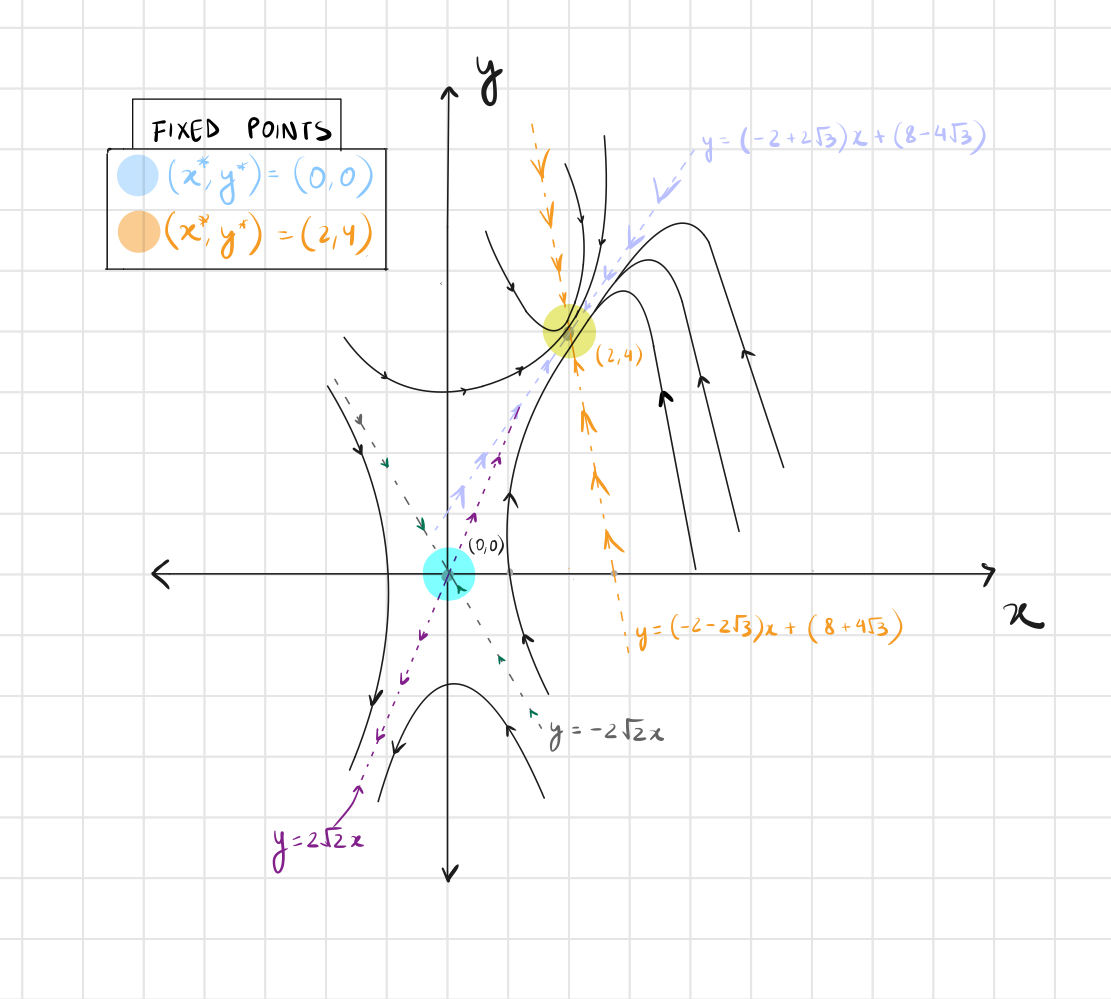
\includegraphics[width=0.9\textwidth]{figures/q2_sketch.jpeg}
    \caption{\centering Phase plane of the system in Eq. 3. The eigenvectors of the Jacobian are plotted in the vicinity of the two fixed points $(x^*,y^*) = (0,0)$ and $(x^*,y^*) = (2,4)$. Various trajectories were plotted qualitatively along these eigenvectors.}
\end{figure}

\newpage
\section*{Question 3: A non-linear model of a chemical replicator with a bifurcation}
It is observed that the system undergoes a bifurcation, with the fixed point at non-zero concentration only
emerging if autocatalysis is fast enough. An alternative model is proposed to explain this behaviour, which
takes the non-dimensionalized form
\begin{align}
    \dot{x} & = \frac{y}{1 + x^2} - x, \nonumber             \\[2pt]
    \dot{y} & = \frac{\epsilon x}{1 + y^2} - y, \label{eq:5}
\end{align}
where $\epsilon$ is a positive constant, and all other parameters that remain after non-dimensionalization have been
assumed to be 1.

\subsubsection*{a. Show that the nullclines of the system are
    $y = x(1 + x^2)$ for $\dot{x} = 0$, and
    $x = \frac{1}{\epsilon} y(1 + y^2)$ for $\dot{y} = 0$.}

To find nullclines, we individually set $\dot{x} = 0$ and $\dot{y} = 0$. To
find the x-nullcline, we set $\dot{x} = 0$:
\begin{align*}
    \dot{x} = 0 \implies \frac{y}{1 + x^2} - x = 0 \implies y = x(1 + x^2)
\end{align*}

To find the y-nullcline, we set $\dot{y} = 0$:
\begin{align*}
    \dot{y} = 0 \implies \frac{\epsilon x}{1 + y^2} - y = 0 \implies x = \frac{1}{\epsilon} y(1 + y^2)
\end{align*}

\subsubsection*{b. This system in above can either have one or two fixed points at physically meaningful values of the variables,
    depending on $\epsilon$. Roughly sketch the form of the nullclines, illustrating both possibilities in separate graphs.}

\begin{figure}[h!]
    \centering
    \begin{minipage}{0.48\textwidth}
        \centering
        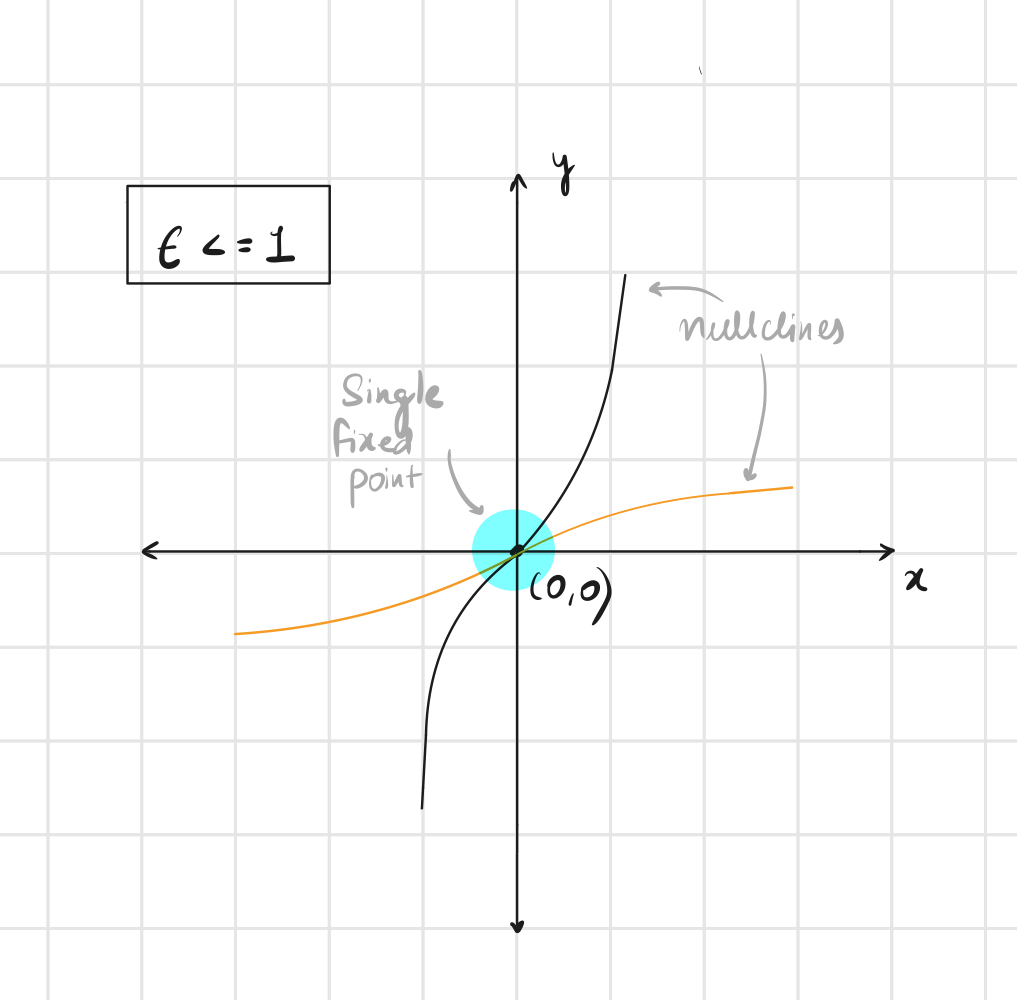
\includegraphics[width=\textwidth]{figures/q3_sketch_2.jpeg}
    \end{minipage}
    % \hfill
    \begin{minipage}{0.48\textwidth}
        \centering
        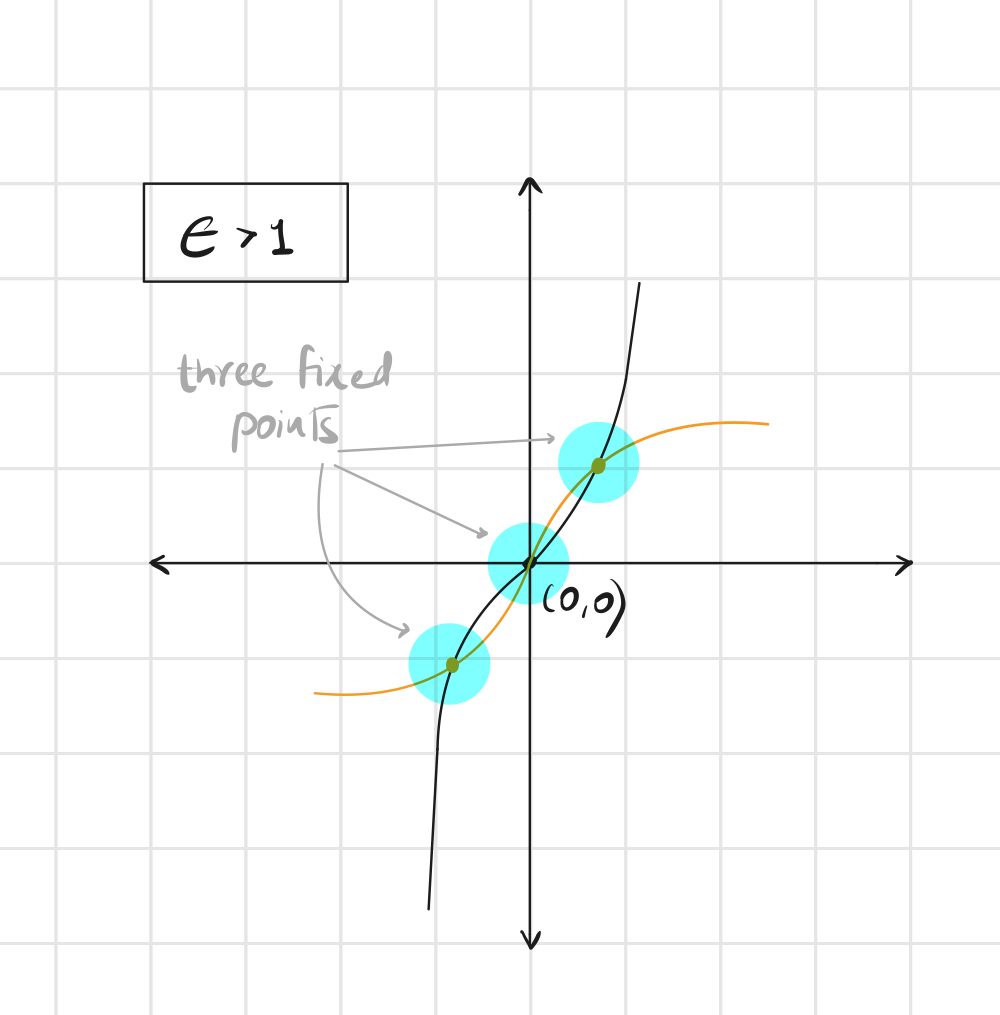
\includegraphics[width=\textwidth]{figures/q3_sketch_1.jpeg}
    \end{minipage}
    \caption{\centering Nullclines of the system for different values of $\epsilon$. Left: When $\epsilon \leq 1$, the nullclines intersect only at the origin, resulting in a single fixed point at $(0,0)$. Right: When $\epsilon > 1$, the nullclines intersect at three points.}
\end{figure}

\newpage
\subsubsection*{c. By considering the gradient of the nullclines in the vicinity of (x,y) = (0,0), or otherwise, show that a
    bifurcation occurs at $\epsilon = 1$. [Hint: you may find it helpful to first calculate $\frac{dx}{dy}$ for the $\dot{y} = 0$ nullcline, and
            then use $\frac{dy}{dx} = 1/\frac{dx}{dy}$]}

To show that a bifurcation occurs at $\epsilon = 1$, let's examine the
gradients of both nullclines near $(0,0)$.

For the x-nullcline ($\dot{x} = 0$): $y = x(1 + x^2)$
\begin{equation*}
    \frac{dy}{dx} = 1 + 3x^2
\end{equation*}
At $(0,0)$: $\left.\frac{dy}{dx}\right|_{(0,0)} = 1$

For the y-nullcline ($\dot{y} = 0$): $x = \frac{1}{\epsilon}y(1 + y^2)$
\begin{align*}
    \frac{dx}{dy} & = \frac{1}{\epsilon}(1 + 3y^2) \\
    \frac{dy}{dx} & = \frac{\epsilon}{1 + 3y^2}
\end{align*}
At $(0,0)$: $\left.\frac{dy}{dx}\right|_{(0,0)} = \epsilon$

For a bifurcation to occur, the nullclines must change their relative
positions. This happens when their gradients at the origin are equal:
\begin{equation*}
    1 = \epsilon \implies \epsilon = 1
\end{equation*}

When $\epsilon < 1$:
\begin{itemize}
    \item The y-nullcline has a smaller gradient than the x-nullcline at the origin
    \item The nullclines intersect only at $(0,0)$
    \item The system has only one fixed point
\end{itemize}

When $\epsilon > 1$:
\begin{itemize}
    \item The y-nullcline has a larger gradient than the x-nullcline at the origin
    \item The nullclines intersect at three points: $(0,0)$ and two symmetric points
    \item The system has three fixed points
\end{itemize}

Therefore, $\epsilon = 1$ is indeed the bifurcation point where the system
transitions from having one to three fixed points.

\subsubsection*{d. Write code to simulate trajectories that start at x = 0.1, y
    = 0 at $\tau$ = 0 and run until $\tau$ = 200. Plot the final value of x against
    $\epsilon$ for $\epsilon$ = (0.55, 0.65, 0.75, 0.85, 0.95, 1.05, 1.15, 1.25,
    1.35, 1.45) to observe the bifurcation.}

\begin{figure}[h]
    \centering
    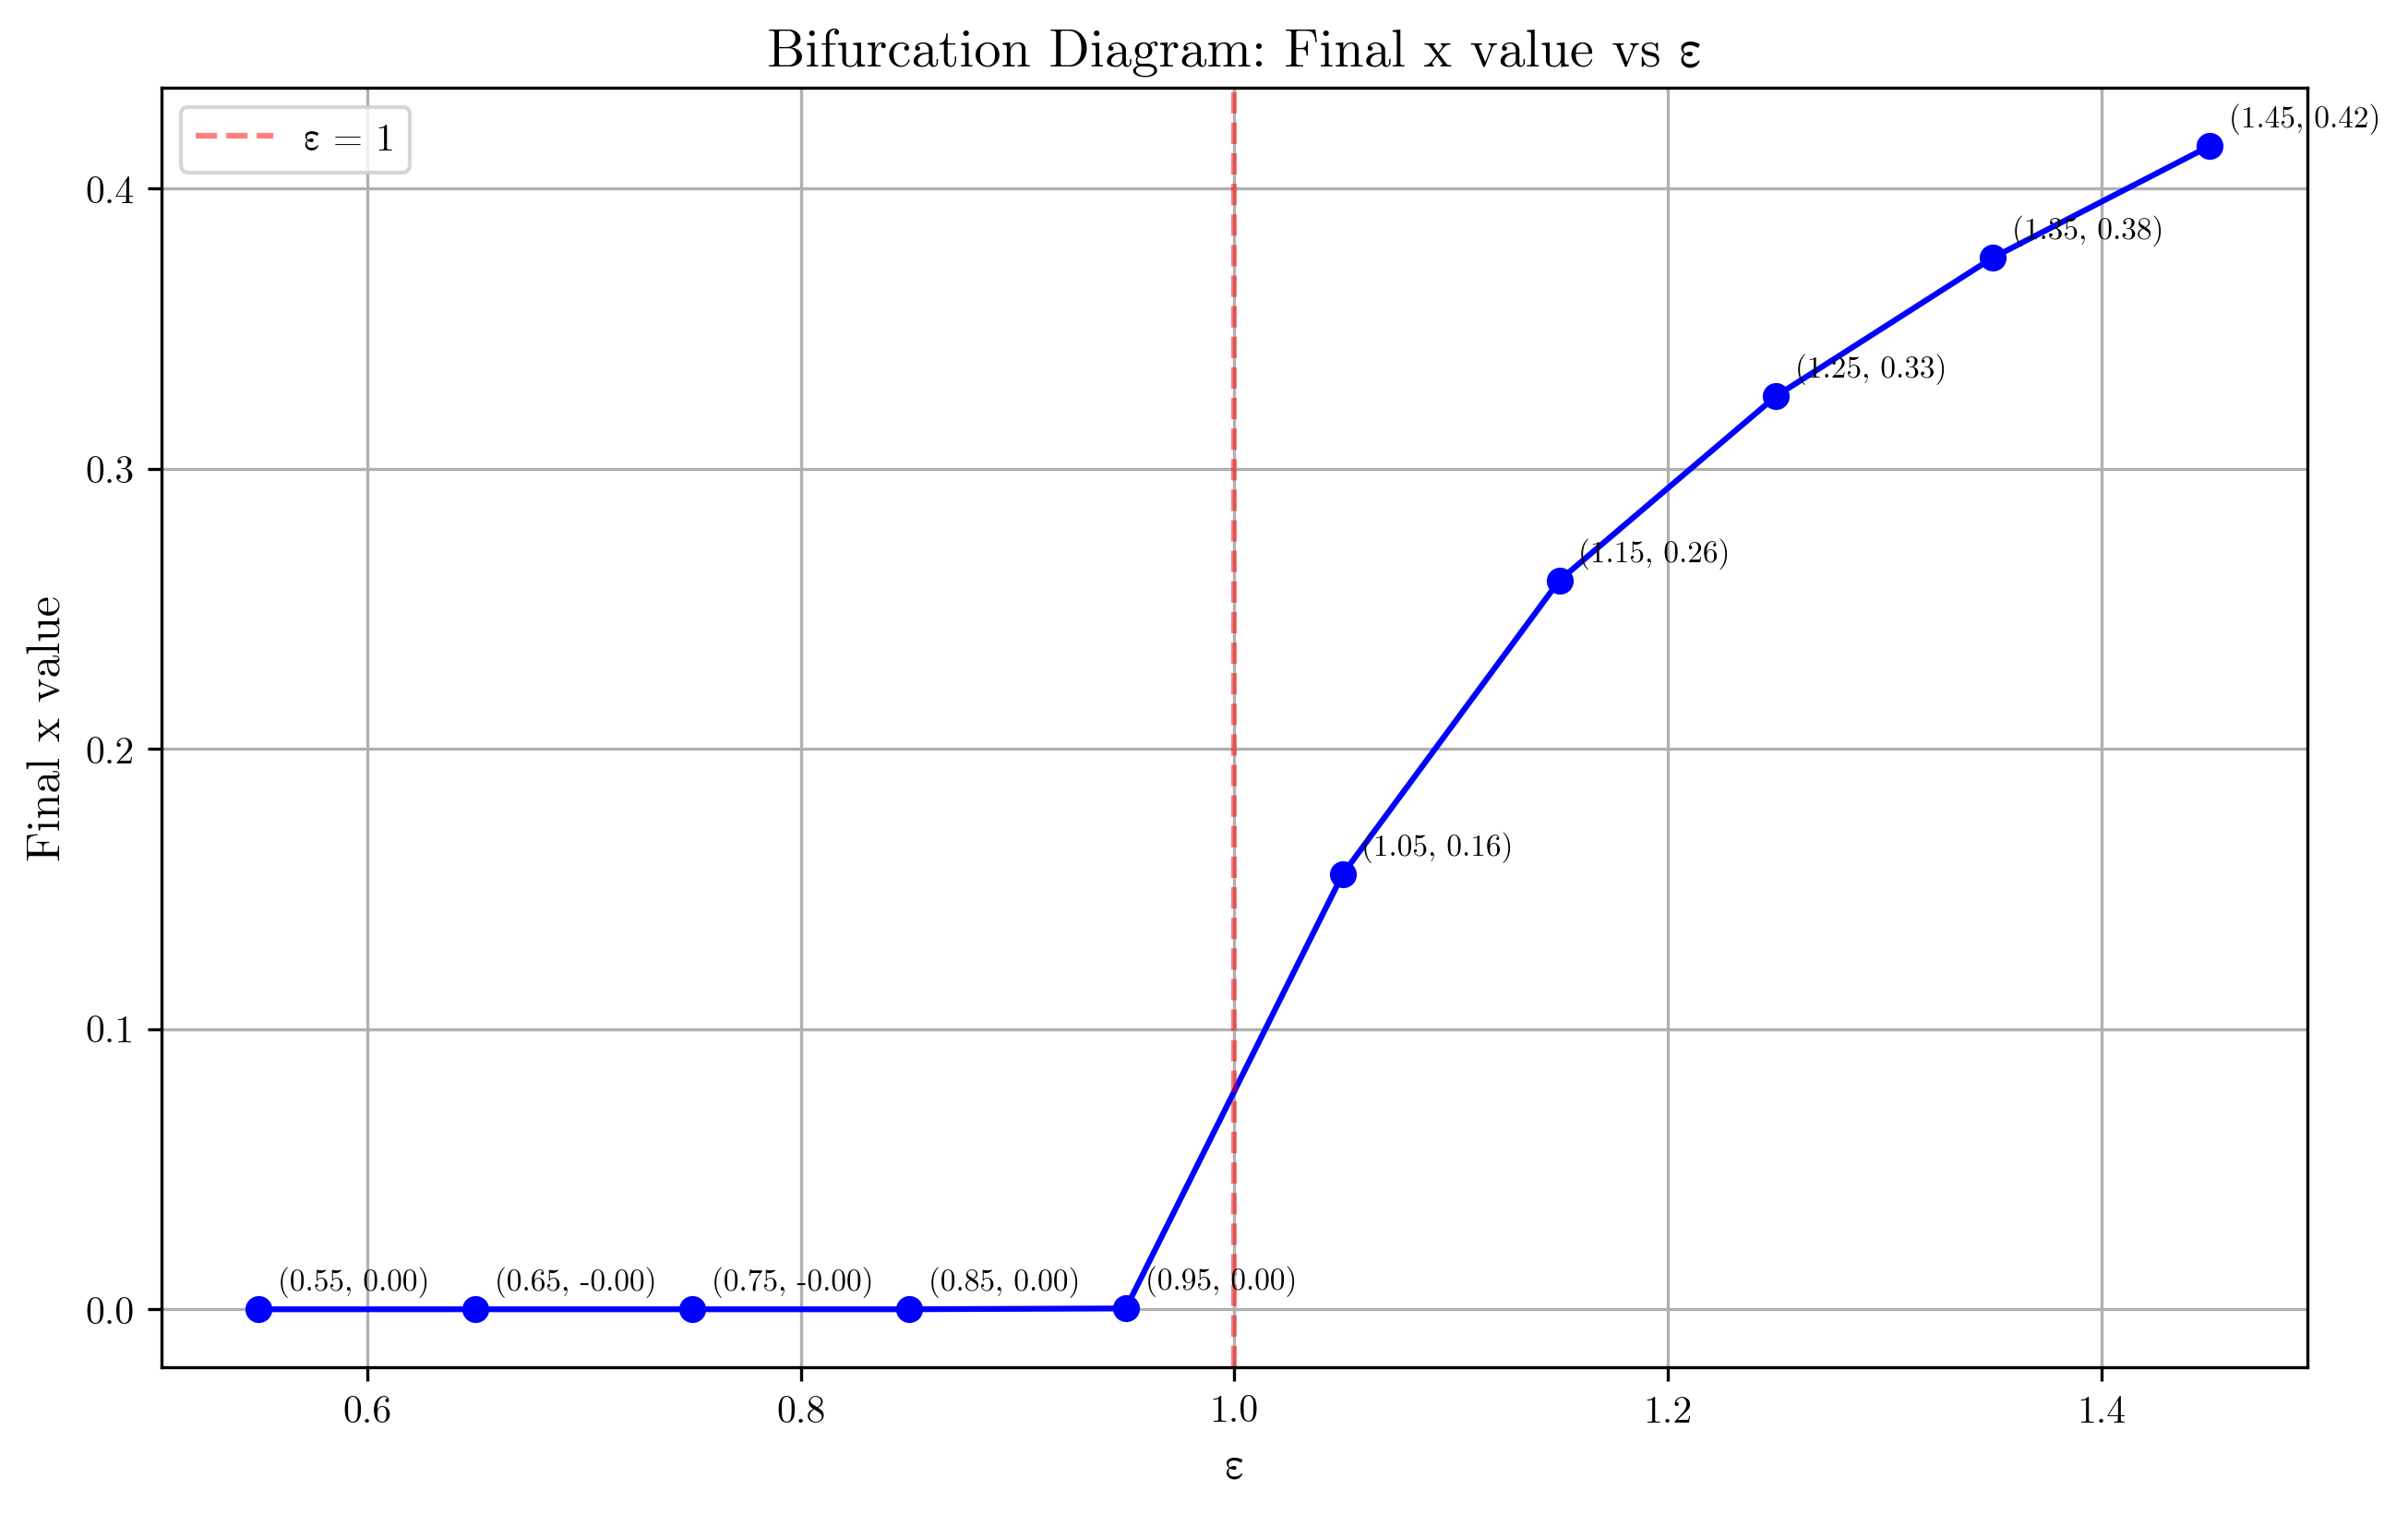
\includegraphics[width=1\textwidth]{figures/q3_plot.png}
    \caption{\centering Bifurcation diagram showing the final value of $x$ at $\tau=200$ for different values of $\epsilon$. For $\epsilon < 1$, the system has only one stable fixed point at the origin. As $\epsilon$ increases past the critical value of 1, a second stable fixed point emerges at non-zero values of $x$, demonstrating bifurcation at $\epsilon = 1$.}
\end{figure}

The code for generating the bifurcation diagram is given below:
\begin{lstlisting}[language=Python, caption=Bifurcation simulation]
import numpy as np
from scipy.integrate import odeint
import matplotlib.pyplot as plt
from matplotlib import font_manager
import matplotlib as mpl

# Load CMU Serif font from file
font_path = '/Users/harshagrawal/Downloads/misc/fonts/cmu-serif/cmunrm.ttf'
font_manager.fontManager.addfont(font_path)
plt.rcParams['font.family'] = 'CMU Serif'
plt.rcParams['mathtext.fontset'] = 'cm'

# Increase DPI for better quality
plt.rcParams['figure.dpi'] = 300
plt.rcParams['savefig.dpi'] = 300

def system(state, t, epsilon):
    x, y = state
    dx_dt = y/(1 + x**2) - x
    dy_dt = (epsilon * x)/(1 + y**2) - y
    return [dx_dt, dy_dt]

# Initial conditions
x0 = 0.1
y0 = 0.0
initial_state = [x0, y0]

# Time points
t = np.linspace(0, 200, 1000)

# Epsilon values
epsilon_values = np.array([0.55, 0.65, 0.75, 0.85, 0.95, 1.05, 1.15, 1.25, 1.35, 1.45])

# Store final x values
final_x_values = []

# Simulate for each epsilon value
for epsilon in epsilon_values:
    # Solve ODE using scipy.integrate.odeint
    solution = odeint(system, initial_state, t, args=(epsilon,))
    
    # Store final x value
    final_x = solution[-1, 0]  # First column is x, take last time point
    final_x_values.append(final_x)

# Plot results
plt.figure(figsize=(10, 6))
plt.plot(epsilon_values, final_x_values, 'bo-')

# Add point labels
for i, (eps, x_val) in enumerate(zip(epsilon_values, final_x_values)):
    plt.annotate(f'({eps:.2f}, {x_val:.2f})', 
                (eps, x_val),
                xytext=(5, 5),
                textcoords='offset points',
                fontsize=8)

plt.grid(True)
plt.xlabel('Epsilon', fontsize=12)
plt.ylabel('Final x value', fontsize=12)
plt.title('Bifurcation Diagram: Final x value vs Epsilon', fontsize=14)

# Add vertical line at Epsilon = 1
plt.axvline(x=1, color='r', linestyle='--', alpha=0.5, label='Epsilon = 1')
plt.legend()

plt.show()
\end{lstlisting}

\end{document}
